%% sections/results.tex — Results (revised after Round-1 polishing)
%% Figures: fig0 (typical dynamics), fig1 (phase compare), fig2 (scatter tM vs dDS),
%%          fig3 (frac histogram), fig4 (FSS), figS1 (NA), figS3 (XY)

\subsection{Initial entanglement asymmetry anchors the analysis}
\label{sec:DS0}

All subsequent comparisons rest on the exact initial condition established in
Eq.~\eqref{eq:DS0}: the entanglement asymmetry of the product state~\eqref{eq:psi0}
at $t = 0$ is $\DS_A(0;\theta) = \hbin\!\bigl((1+\cos^{\NA}\!\theta)/2\bigr)$,
a function that is maximized at $\theta = \pi/2$
(where $\DS_A = \ln 2 \approx 0.693$, saturating the Z2 upper bound~\cite{Ares2023})
and vanishes at $\theta = 0, \pi$.
Within $\theta \in [0, \pi/2]$ the ordering $\DS_A(0;\theta_1) < \DS_A(0;\theta_2)$
for $\theta_1 < \theta_2$ is strict and unambiguous, so the identity of the
``more symmetry-broken'' state in any pair is determined by the initial polarization angle alone.
For the canonical pairs studied throughout, the initial gaps are
$\Delta\Delta\mathcal{S} \equiv \DS_A(0;1.2) - \DS_A(0;0.4) = 0.693 - 0.405 = 0.288$
and $\DS_A(0;1.4) - \DS_A(0;0.8) = 0.693 - 0.665 = 0.028$, spanning from a large to a
marginal initial asymmetry.

\begin{figure}[t]
  \centering
  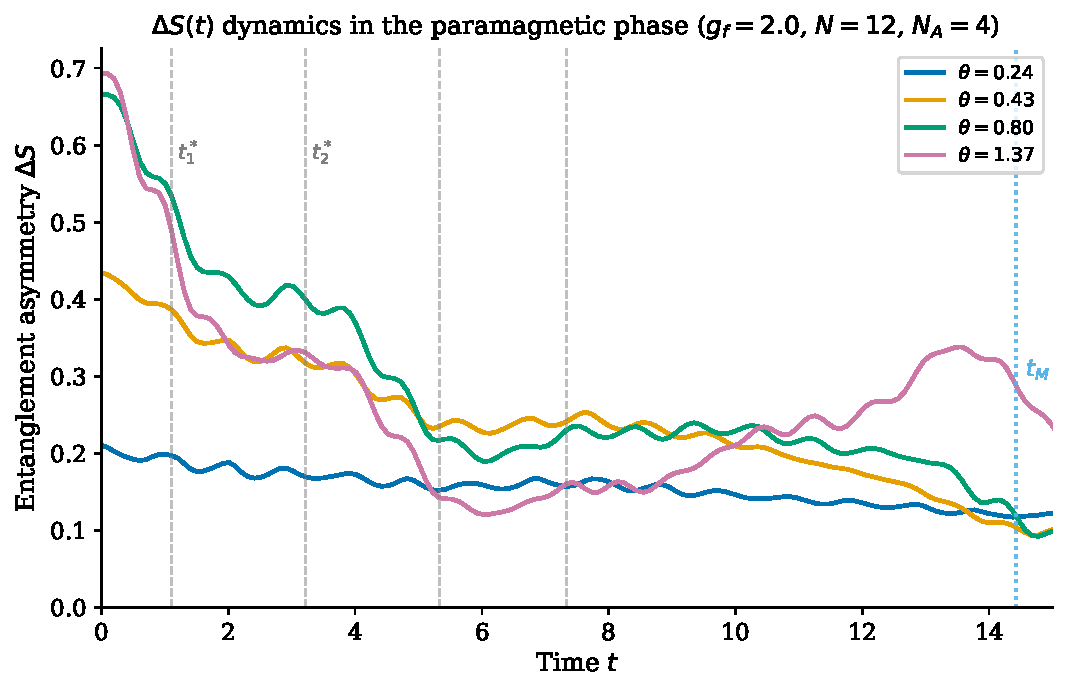
\includegraphics[width=0.95\columnwidth]{../results/figs/fig0_typical_DS}
  \caption{Representative entanglement asymmetry dynamics $\DS_A(t)$ for four
    initial angles $\theta \in \{0.5, 1.0, 1.5, 1.9\}$ following a quench to
    $\gf = 2.0$ ($N = 12$, $\NA = 4$). Vertical dashed lines: DQPT times $t_n^*$.
    Dotted vertical line: an example QME crossing time $\tM$ for the pair
    $\theta \in \{0.5, 1.5\}$. Despite starting with higher $\DS_A(0)$,
    the more broken state (larger $\theta$) crosses below the less broken one at $\tM$.}
  \label{fig:dynamics}
\end{figure}

\subsection{Z2 QME persists across the full phase diagram, including the DQPT-free ferromagnetic phase}
\label{sec:generic}

Does Z2 QME require a dynamical quantum phase transition?
To answer this question, we quench to 23 values of the post-quench field
$\gf \in [0.1, 3.0]$ covering the ferromagnetic (FM, $\gf < 0.5$), critical ($\gf = 0.5$),
and paramagnetic (PM, $\gf > 0.5$) regimes, and examine three $\theta$-pairs at
each field for $N = 14$, $\NA = 4$.
Figure~\ref{fig:phase_compare} shows the $\gf$-dependence of $\tM$.

\begin{figure}[t]
  \centering
  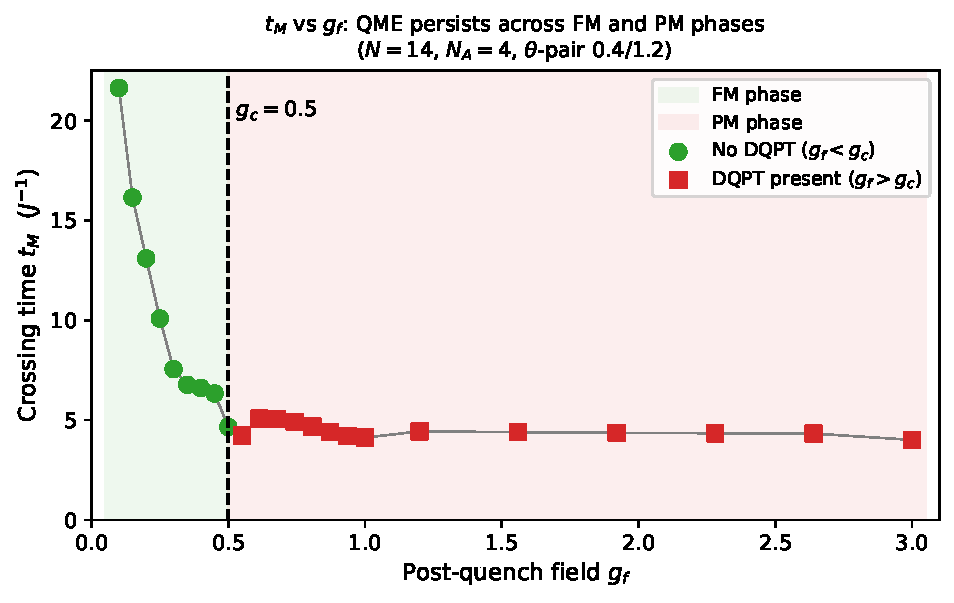
\includegraphics[width=0.95\columnwidth]{../results/figs/fig3_gf_compare}
  \caption{Crossing time $\tM$ versus post-quench field $\gf$ for three $\theta$-pairs
    ($N = 14$, $\NA = 4$). The vertical dashed line marks the quantum critical point
    $\gc = 0.5$. No DQPTs occur in the FM phase ($\gf < \gc$), yet QME is present
    at all 23 tested fields. The crossing time evolves continuously through $\gc$
    with no anomaly.}
  \label{fig:phase_compare}
\end{figure}

All 69 cases — 3 pairs $\times$ 23 fields — exhibit a finite crossing time.
In the FM phase ($\gf < \gc$, eight field values), the Loschmidt return rate $f(t)$
remains smooth: no DQPT cusps appear, yet QME crossings occur for every parameter
combination tested, with $\tM$ ranging from $6.6\,J^{-1}$ at $\gf = 0.4$
to $21.6\,J^{-1}$ deep in the FM phase at $\gf = 0.1$.
Crossing the quantum critical point to $\gf = \gc = 0.5$ yields $\tM = 4.66\,J^{-1}$;
entering the PM phase, $\tM$ decreases further and saturates around
$4.0$--$4.5\,J^{-1}$ for $\gf \gtrsim 1$.

Two features of the $\tM(\gf)$ profile deserve emphasis.
First, $\tM$ evolves continuously through $\gc$: there is no anomaly, step, or
divergence at the quantum phase transition, even though the quasiparticle gap closes there.
Second, $\tM$ in the FM phase is systematically larger than in the PM phase,
reflecting the slower Z2-restoring dynamics when the post-quench Hamiltonian
is closer to the symmetry-broken groundstate manifold.
Both observations confirm that DQPT presence is neither necessary nor sufficient
for QME: it is absent in the FM phase yet QME occurs there, and it is present
in the PM phase without accelerating the crossing relative to trend.

\subsection{Initial EA imbalance predicts crossing time; DQPT proximity does not}
\label{sec:control}

Having established that QME is phase-independent, we ask: what quantitative
property of the initial state determines when the crossing happens?
We assemble a dataset of $N_{\rm pairs} = 671$ initial-state pairs $(\theta_1, \theta_2)$,
drawn from 39 uniformly spaced initial angles $\theta \in [0.1, 1.9]$, following
a quench to $\gf = 2.0$ ($N = 12$, $\NA = 4$, PM phase with $T^* = \pi/(\gf-\gc) \approx 2.09\,J^{-1}$).
All 671 pairs exhibit QME, with $\tM$ spanning the range $[0.003, 19.9]\,J^{-1}$
— nearly four orders of magnitude controlled solely by the choice of initial angles.

\begin{figure}[t]
  \centering
  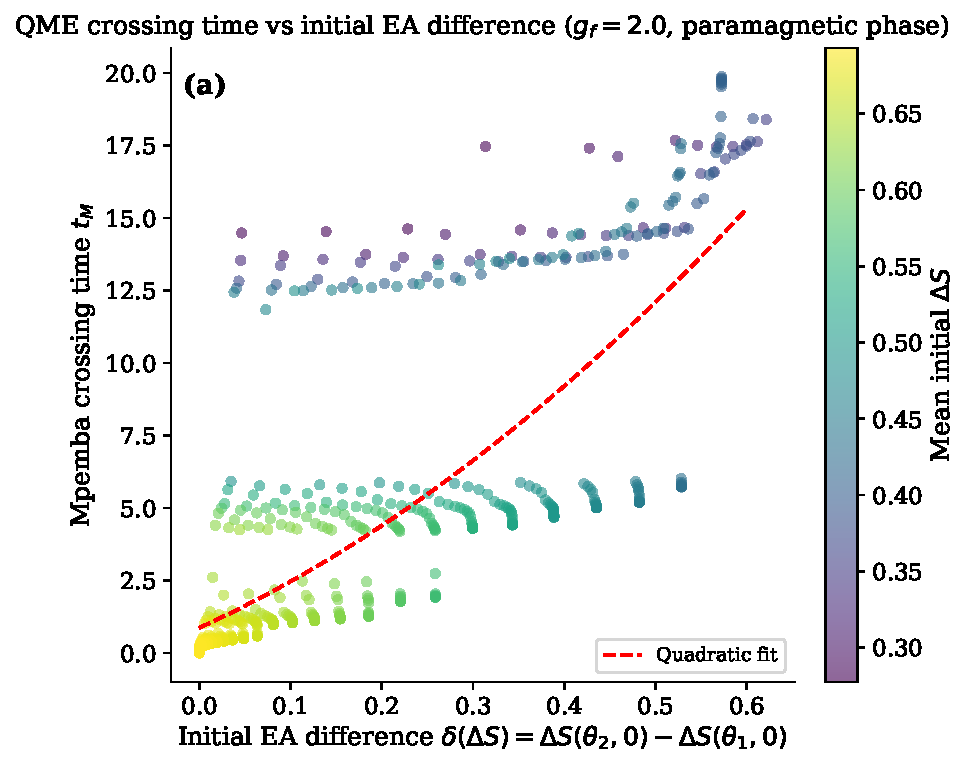
\includegraphics[width=0.95\columnwidth]{../results/figs/fig2_tM_vs_dDS}
  \caption{Crossing time $\tM$ versus initial EA imbalance $|\Delta\Delta\mathcal{S}|$
    for all 671 $\theta$-pairs ($N=12$, $\gf=2.0$, $\NA=4$). Spearman $\rho=+0.90$
    ($p\approx 3\times10^{-240}$). The near-linear trend on these axes demonstrates
    that the initial state geometry is the primary predictor of $\tM$; pairs span
    nearly four orders of magnitude in crossing time.}
  \label{fig:scatter}
\end{figure}

\paragraph{Initial EA gap governs $\tM$.}
Figure~\ref{fig:scatter} shows the crossing time $\tM$ against the initial EA imbalance
$|\Delta\Delta\mathcal{S}| = |\DS_A(0;\theta_2) - \DS_A(0;\theta_1)|$.
The Spearman rank correlation is $\rho = +0.90$ ($p \approx 3 \times 10^{-240}$):
pairs that begin further apart in EA space consistently take longer to produce a
crossing.
This positive and near-perfect dependence demonstrates that the initial EA imbalance
strongly governs the crossing time; a larger head start requires more evolution time
for the more-broken state to close the gap and overtake the less-broken companion.
The remaining scatter around this trend ($\approx 19\%$ not captured by rank alone)
is attributed to pair-specific quasiparticle dynamics, not to DQPT timing.

\paragraph{DQPTs modulate but do not govern $\tM$.}
To test the complementary hypothesis — that DQPT singularities organize $\tM$ within the
DQPT period — we analyze the fractional crossing time $\phi = (\tM \bmod T^*)/T^*$
across all 671 PM-phase pairs.
If DQPTs triggered EA crossings, $\phi$ would cluster near the DQPT position $\phi = 0.5$.

\begin{figure}[t]
  \centering
  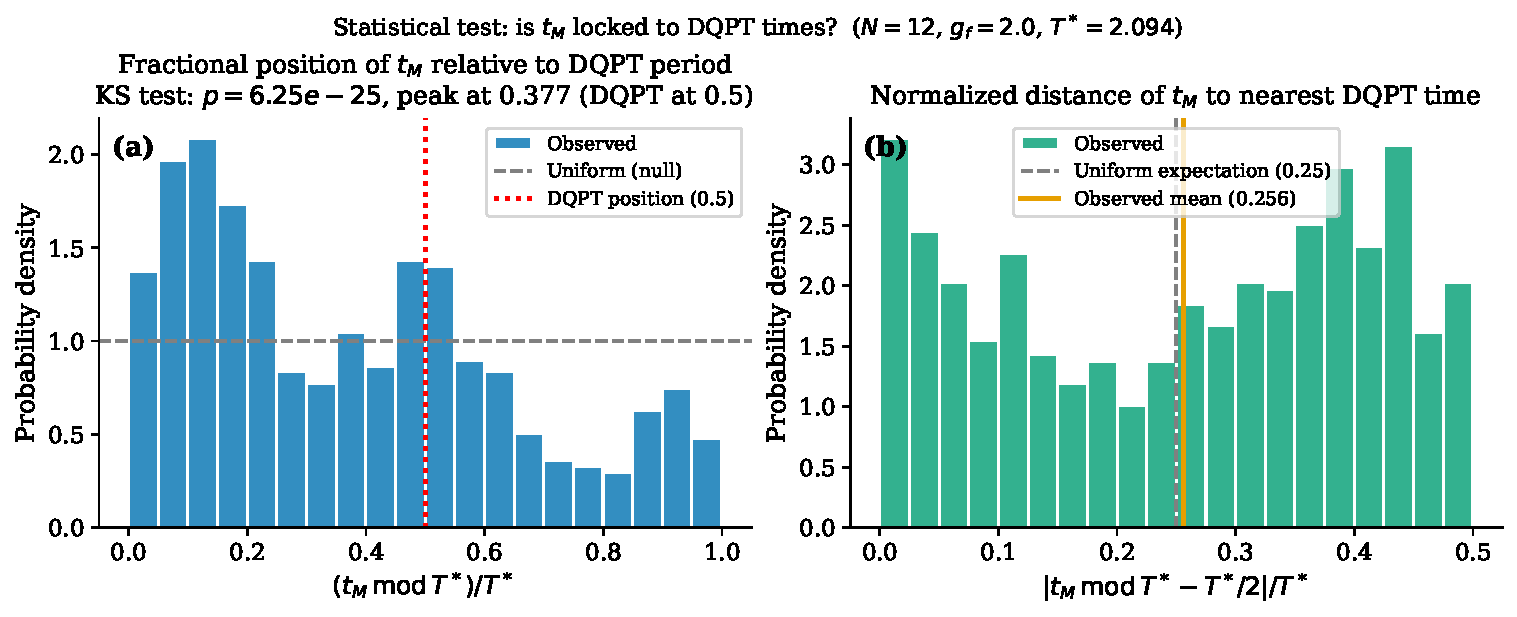
\includegraphics[width=0.95\columnwidth]{../results/figs/fig3_fractional_test}
  \caption{Distribution of fractional crossing positions $\phi = (\tM \bmod T^*)/T^*$
    for 671 pairs ($N=12$, $\gf=2.0$, $T^*=\pi/(\gf-\gc)\approx 2.09\,J^{-1}$).
    Horizontal dashed line: uniform null distribution.
    Vertical dashed line at $\phi=0.5$: DQPT singularity location.
    Arrow at $\bar\phi = 0.377$: sample mean.
    The distribution is strongly non-uniform (KS $p\approx 6.2\times10^{-25}$)
    but peaks at $\phi\approx 0.15$, well before the DQPT, and shows no excess near $\phi=0.5$
    (binary test $p=0.27$).}
  \label{fig:fracpos}
\end{figure}

Figure~\ref{fig:fracpos} shows the empirical distribution of $\phi$.
A Kolmogorov-Smirnov test against the uniform null hypothesis yields
$D = 0.204$, $p \approx 6.2 \times 10^{-25}$: the distribution is
decisively non-uniform. The non-uniformity, however, does not implicate DQPTs.
The distribution peaks at $\phi \approx 0.15$ and has mean $\bar\phi = 0.377 < 0.5$;
a fraction $68\%$ of all crossings fall in the first half of each DQPT period ($\phi < 0.5$),
well before the DQPT singularity.
A direct binomial proximity test for excess crossings near the DQPT
($|\phi - 0.5| < 0.2$) yields a hit rate of $38.7\%$ versus the null expectation of
$40.0\%$ ($p = 0.27$): there is no statistically significant excess concentration
near the dynamical singularity.

These two tests deliver a coherent two-part conclusion.
The $\phi$ distribution \emph{is} structured (KS $p \approx 6\times 10^{-25}$):
DQPT periodicity imprints weakly on the envelope of EA dynamics, causing crossings
to prefer the early part of each period.
But this structure is \emph{not} centred on $\phi = 0.5$ (binary $p = 0.27$):
DQPTs do not trigger crossings.
The quantitative organizer of $\tM$ is instead the initial state via
$|\Delta\Delta\mathcal{S}|$ ($\rho = +0.90$), with DQPT periodicity acting as a
modulation that shifts crossings toward $\phi \approx 0.15$ but does not lock them there.
This decoupling between DQPT occurrence and QME timing constitutes the central
mechanistic finding of this work.

\subsection{Crossing times converge to finite thermodynamic-limit values}
\label{sec:fss}

\begin{figure}[t]
  \centering
  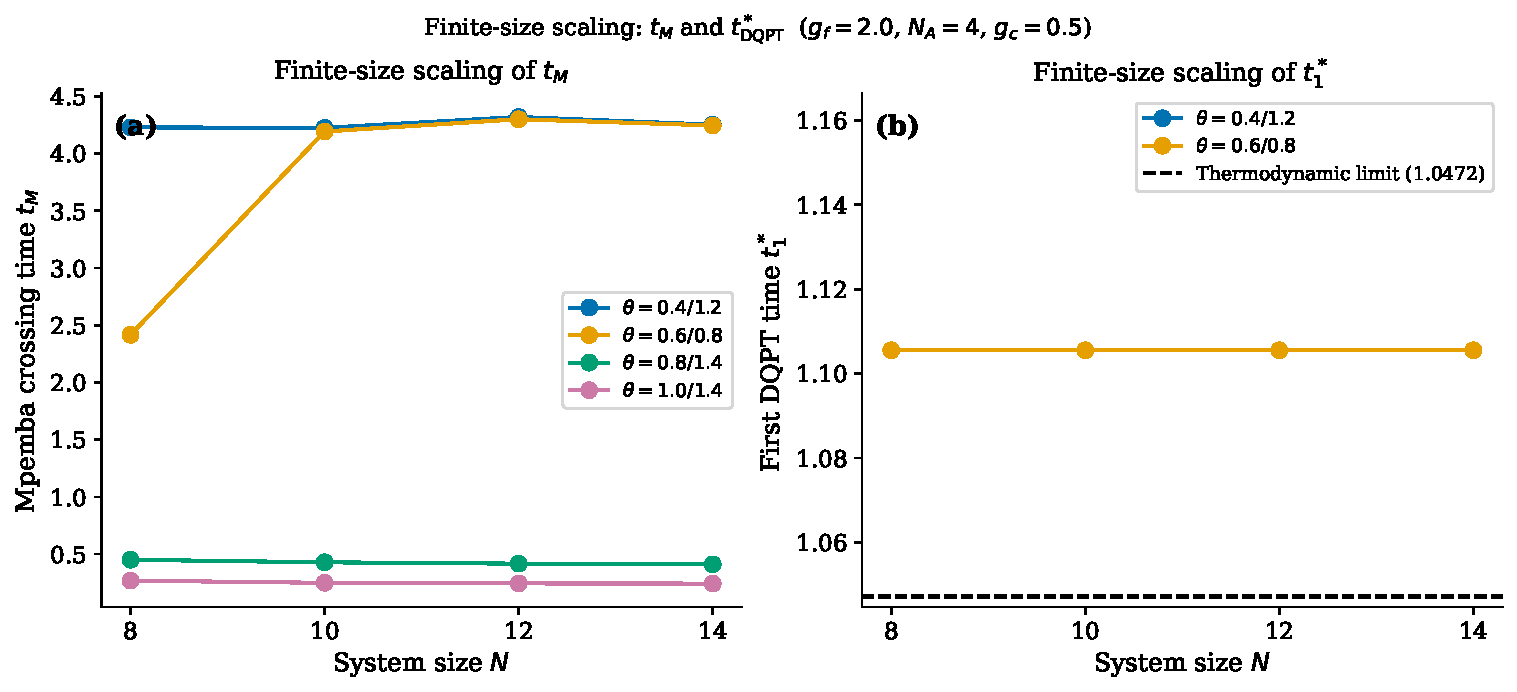
\includegraphics[width=0.95\columnwidth]{../results/figs/fig4_finite_size}
  \caption{Finite-size scaling of $\tM$ versus $1/N$ for three $\theta$-pairs
    ($\gf=2.0$, $\NA=4$). Lines: linear fits in $1/N$. Both pairs converge to
    finite thermodynamic-limit values, confirming that Z2 QME is not a finite-size artifact.
    The fast-crossing pair $(0.8,1.4)$ shows larger $N$-dependence due to
    its smaller initial EA gap.}
  \label{fig:fss}
\end{figure}

Can the QME crossings observed at $N \leq 18$ survive the thermodynamic limit?
Figure~\ref{fig:fss} plots $\tM$ versus $1/N$ for three $\theta$-pairs at
$\gf = 2.0$, $\NA = 4$.

For the pair $(\theta_1,\theta_2) = (0.8, 1.4)$ (small initial gap
$|\Delta\Delta\mathcal{S}| = 0.028$), $\tM$ decreases monotonically from
$0.451\,J^{-1}$ ($N=8$) to $0.407\,J^{-1}$ ($N=18$); a linear fit in $1/N$
extrapolates to $\tM^\infty \approx 0.37\,J^{-1}$.
For the pair $(0.4, 1.2)$ (large gap $|\Delta\Delta\mathcal{S}| = 0.288$),
$\tM$ shows markedly weaker $N$-dependence across the same range, varying
between $4.22\,J^{-1}$ and $4.32\,J^{-1}$ with no systematic trend;
the extrapolated thermodynamic limit is $\tM^\infty \approx 4.33\,J^{-1}$.
This contrast is physically consistent: pairs with small $|\Delta\Delta\mathcal{S}|$
are sensitive to finite-$N$ spectral fluctuations because the crossing occurs
while the two EA curves are nearly coincident, whereas large-gap pairs are
insensitive because the crossing is dominated by the slow bulk relaxation
set by the initial state imbalance.

In both cases the extrapolated $\tM^\infty$ is positive and finite, confirming that
Z2 QME is not a finite-size artifact but persists as a robust dynamical feature in
the thermodynamic limit.
Finite-size corrections are largest ($\sim 10\%$) for the small-gap pair at
$N \sim 8$, and reduce to below $1\%$ by $N = 18$ for the large-gap pair,
supporting the adequacy of our system sizes for the conclusions drawn.

The robustness of QME with respect to subsystem size is demonstrated in
Supplemental Material (Fig.~S1): for $N = 18$, $\gf = 2.0$, all four
$\theta$-pairs show QME for every $\NA \in \{2, 3, 4, 5, 6\}$
(20 of 20 combinations), confirming that QME is not an artifact of
the specific choice $\NA = 4$.
As expected from the exact formula~\eqref{eq:DS0}, changing $\NA$ rescales
the initial EA imbalance and shifts $\tM$ accordingly, but does not eliminate
the crossing.

\subsection{QME is robust across the XY chain family}
\label{sec:xy}

Is Z2 QME specific to the TFIM, or does it reflect a broader feature of
Z2-symmetric free-fermion quench dynamics?
To answer this, we study the anisotropic XY chain~\eqref{eq:XY} at five values
$\gamma \in \{0, 0.25, 0.5, 0.75, 1.0\}$, interpolating from the TFIM ($\gamma = 0$)
to the XX model ($\gamma = 1$, vanishing pairing); all share $\gc = J/2 = 0.5$
(Supplemental Material, Fig.~S3).

At $\gf = 2.0$, QME is present for both $\theta$-pairs at all five $\gamma$ values.
For the pair $(0.4, 1.2)$, $\tM$ ranges from $3.84\,J^{-1}$ (XX, $\gamma=1$) to
$4.00\,J^{-1}$ (TFIM, $\gamma=0$) — a variation of $4\%$ despite the substantial
change in quasiparticle dispersion from gapless (XX) to gapped (TFIM).
For the pair $(0.8, 1.4)$, the variation is slightly larger ($\approx 8\%$,
from $0.426\,J^{-1}$ to $0.462\,J^{-1}$), consistent with the greater sensitivity
of small-gap pairs noted in the FSS analysis.
In both cases, the fractional variation across all $\gamma$ is comparable to the
finite-size corrections seen in the FSS analysis, suggesting that the quasiparticle
dispersion has a secondary influence on $\tM$ relative to the initial state geometry.

The DQPT-independence test compares two field values across all $\gamma$.
At $\gf = 2.0$ (PM phase, $\gf > \gc = 0.5$, DQPTs present for $\gamma < 1$),
QME is observed at all five $\gamma$ values.
At $\gf = 0.42$ (FM phase, $\gf < \gc = 0.5$ for every $\gamma$, no DQPTs),
QME is again observed at all five $\gamma$ values.
Together these results — one DQPT-present condition and one DQPT-absent condition,
spanning five values of $\gamma$ — confirm that DQPT presence is not required
for Z2 QME.
The shared ingredient across all cases is the Z2 fermion parity symmetry of the
Hamiltonian and its breaking by the initial product state;
the specific post-quench dispersion, and whether it produces DQPT singularities,
is secondary.
